%yright 2007, 2008, 2009 Elsevier Ltd
%% 
%% This file is part of the 'Elsarticle Bundle'.
%% ---------------------------------------------
%% 
%% It may be distributed under the conditions of the LaTeX Project Public
%% License, either version 1.2 of this license or (at your option) any
%% later version.  The latest version of this license is in
%%    http://www.latex-project.org/lppl.txt
%% and version 1.2 or later is part of all distributions of LaTeX
%% version 1999/12/01 or later.
%% 
%% The list of all files belonging to the 'Elsarticle Bundle' is
%% given in the file `manifest.txt'.
%% 

%% Template article for Elsevier's document class `elsarticle'
%% with numbered style bibliographic references
%% SP 2008/03/01

% \documentclass[preprint,11pt]{elsarticle}
\documentclass[final,1p,11pt]{elsarticle}

%\documentclass[final,1p,times]{elsarticle}


%% Use the option review to obtain double line spacing
%%\documentclass[authoryear,preprint,review,12pt]{elsarticle}

%% Use the options 1p,twocolumn; 3p; 3p,twocolumn; 5p; or 5p,twocolumn
%% for a journal layout:
%% \documentclass[final,1p,times]{elsarticle}
%% \documentclass[final,1p,times,twocolumn]{elsarticle}
%% \documentclass[final,3p,times]{elsarticle}
%% \documentclass[final,3p,times,twocolumn]{elsarticle}
%% \documentclass[final,5p,times]{elsarticle}
%% \documentclass[final,5p,times,twocolumn]{elsarticle}

%%% For including figures, graphicx.sty has been loaded in
%% elsarticle.cls. If you prefer to use the old commands
%% please give \usepackage{epsfig}


\usepackage{epsfig}
%\usepackage{cite}
%\usepackage{mcite}
\usepackage{array,tabularx,epsfig,mathrsfs,graphicx,rotating}
\usepackage{ifthen}
\usepackage{amsfonts}
\usepackage{ragged2e}
\PassOptionsToPackage{hyphens}{url}
\usepackage[hyphens]{url}
\usepackage{hyperref}
\usepackage{listings}
\usepackage{lineno}
\usepackage{subfigure}
\usepackage{epstopdf}
% Custom colors
\usepackage{color}
\usepackage{float}
\usepackage{verbatim}
\usepackage{color,soul}
\usepackage{subfigure} 


% to cross text
\usepackage[normalem]{ulem} % either use this (simple) or
\usepackage{soul} % use this (many fancier options)
\usepackage{amsmath,amssymb}

\let\originallesssim\lesssim
\let\originalgtrsim\gtrsim

\DeclareRobustCommand{\lesssim}{%
  \mathrel{\mathpalette\lowersim\originallesssim}%
}
\DeclareRobustCommand{\gtrsim}{%
  \mathrel{\mathpalette\lowersim\originalgtrsim}%
}

\makeatletter
\newcommand{\lowersim}[2]{%
  \sbox\z@{$#1<$}%
  \raisebox{-\dimexpr\height-\ht\z@}{$\m@th#1#2$}%
}
\makeatother


\hypersetup{
  colorlinks=true,
  linkcolor=blue,
  citecolor=blue,
  urlcolor=blue
}




\graphicspath{{figs/}}


\pdfinfo{
   /Author (Chekanov et al)
   /Title  (Physics potential of timing layers for future detectors)
   /CreationDate (D:2020)
   /Subject (PDFLaTeX)
   /Keywords (PDF;LaTeX)
}


\textheight=22cm
\textwidth=14.5cm

\newcommand{\beq}{\begin{equation}}
\newcommand{\eeq}{\end{equation}}
\newcommand{\la}{\langle}
\newcommand{\promc}{{\sc ProMC}}
\newcommand{\ra}{\rangle}
\newcommand{\eps}{\epsilon}
\newcommand{\ud}{\mathrm{d}}
\newcommand{\Ec}{\mathcal{E}}
\newcommand{\Fc}{\mathcal{F}}
\newcommand{\Za}{\mathrm{Z_1}}
\newcommand{\Zb}{\mathrm{Z_2}}
\newcommand{\Zn}{\mathrm{Z_n}}
\newcommand{\F}{\mathrm{F}}

\chardef\til=126
\newcommand{\GEANTfour} {\textsc{geant4}}
\newcommand{\pythia} {\textsc{Pythia8~}}
\newcommand{\pt}{\ensuremath{p_{\mathrm{T}}}}


\journal{}

\begin{document}
%\hfill ANL-HEP-149528
\definecolor{mygreen}{rgb}{0,0.6,0} \definecolor{mygray}{rgb}{0.5,0.5,0.5} \definecolor{mymauve}{rgb}{0.58,0,0.82}

\lstset{ %
 backgroundcolor=\color{white},   % choose the background color; you must add \usepackage{color} or \usepackage{xcolor}
 basicstyle=\footnotesize,        % the size of the fonts that are used for the code
 breakatwhitespace=false,         % sets if automatic breaks should only happen at whitespace
 breaklines=true,                 % sets automatic line breaking
 captionpos=b,                    % sets the caption-position to bottom
 commentstyle=\color{mygreen},    % comment style
 deletekeywords={...},            % if you want to delete keywords from the given language
 escapeinside={\%*}{*)},          % if you want to add LaTeX within your code
 extendedchars=true,              % lets you use non-ASCII characters; for 8-bits encodings only, does not work with UTF-8
 keepspaces=true,                 % keeps spaces in text, useful for keeping indentation of code (possibly needs columns=flexible)
 frame=tb,
 keywordstyle=\color{blue},       % keyword style
 language=Python,                 % the language of the code
 otherkeywords={*,...},            % if you want to add more keywords to the set
 rulecolor=\color{black},         % if not set, the frame-color may be changed on line-breaks within not-black text (e.g. comments (green here))
 showspaces=false,                % show spaces everywhere adding particular underscores; it overrides 'showstringspaces'
 showstringspaces=false,          % underline spaces within strings only
 showtabs=false,                  % show tabs within strings adding particular underscores
 stepnumber=2,                    % the step between two line-numbers. If it's 1, each line will be numbered
 stringstyle=\color{mymauve},     % string literal style
 tabsize=2,                        % sets default tabsize to 2 spaces
 title=\lstname,                   % show the filename of files included with \lstinputlisting; also try caption instead of title
 numberstyle=\footnotesize,
 basicstyle=\small,
 basewidth={0.5em,0.5em}
}

% linenumbers
\linenumbers


\begin{frontmatter}

\title{
Physics potential of timing layers for future detectors}
%%%%%%%%%%%%%%%%%%%%%%%%%%%%%%%%%%%%%%%%%%%%%%%%%%%%%%%%%%%%%%%

\author[add1]{S.V.~Chekanov}
\ead{chekanov@anl.gov}

\author[addDuke]{A.V.~Kotwal}
\ead{ashutosh.kotwal@duke.edu}

\author[add3]{C.-H. Yeh}
\ead{a9510130375@gmail.com}


\author[add3]{S.-S.~Yu}
\ead{syu@cern.ch}

\address[add1]{
HEP Division, Argonne National Laboratory,
9700 S.~Cass Avenue,
Argonne, IL 60439, USA.
}


\address[add3]{
Department of Physics and Center for High Energy and High Field Physics, 
National Central University, Chung-Li, Taoyuan City 32001, Taiwan
}

\address[addDuke]{
Department of Physics, Duke University, USA
}


\begin{abstract}
The physics potential of timing layers with a few tens of pico-second resolution for 
calorimeters of future detectors in collider experiments is explored.
The presented studies show how such layers can be used for identification 
of separate particles,  as well as illustrate the benefit of detecting  
new event signatures beyond  the Standard Model. 
\end{abstract}

\begin{keyword}

\end{keyword}
\end{frontmatter}



%%%%%%%%%%%%%%%%%%%%%%%%%%%%%%%%%%%%%%%%%%%%%%%%%%%%%%%%%%%%%%%%%%
\section{Introduction}

Future experiments, such as CLIC \cite{Linssen:1425915}, International Linear Collider (ILC) \cite{Behnke:2013xla}, high-energy LHC (HE-LHC),
future circular $pp$ colliders of the European initiative, FCC-hh~\cite{Benedikt:2206376} and the Chinese initiative, SppC~\cite{Tang:2015qga} 
will require high precision measurements of particles and jets 
at large transverse momenta. 
The usage of timing information for such experiments  can  provide additional 
information that can be used to improve particle and jet reconstruction, as well as to reduce background events.
For example, high-precision timing will be beneficial for b-tagging for all post-LHC experiments. 
For CLIC and FCC, high-precision time stamping of calorimeter energy deposits will be essential for
background rejection (i.e. fake energy deposits) and pile-up mitigation.
Precise timing information is important for improving reconstruction of particle flow objects by reducing overlap 
of energy showers in highly-granular calorimeters.

From the physics point of view, timing layers can be used for detection of long-lived particles and identification 
of standard model (SM) particles. 
At this moment, conceptional design reports for future experiments have not yet fully explored 
the benefits of the time of flight (TOF) measurements with tens-of-picosecond resolutions for calorimeters.

In this paper we will investigate the benefits of the timing layers with the resolution in the range
10~ps -- 1~ns for identification of SM particles. 
The resolution of 1~ns is standard for the existing and planned calorimeters \cite{Linssen:1425915,Behnke:2013xla,Benedikt:2206376,Tang:2015qga}, 
and is only used as a benchmark for comparisons with more challenging  
10 -- 20~ps  resolution devices. 
In addition, we investigate the capabilities of timing layers for identification of heavy stable particles which may be produced beyond the 
standard model (BSM). We hope such studies can help shape the requirements for future calorimeters, which were already
outlined in the CPAD report \cite{Ahmed:2019sim} that emphasized the need to develop fast timing readout for calorimeter measurements.
  
%%%%%%%%%%%%%%%%%%%%%%%%%%%%%%
\section{Proposal}
%%%%%%%%%%%%%%%%%%%%%%%%%%%%%


A generic design of hadronic (electromagnetic) calorimeters for future particle collision experiments (HE-LHC, FCC, CLIC, ILC etc.) 
is based on two main characteristics: (1) high-granularity  electromagnetic (ECAL) and hadronic (HCAL) 
calorimeters with cells ranged from $3\times 3$~mm$^2$ to $5\times 5$~cm$^2$.
(2) timing with a nanosecond precision that improves background rejection, vertex association, and detection of new particles. 
According to the CPAD report \cite{Ahmed:2019sim}, a development of ``picosecond time resolution'' for future calorimeters is one of the critical needs. 
Presently,  high-granularity calorimeters with $>1$ millions channels and with tens of pico-second resolution represent a 
significant challenge due to the large cost.

As a part of the HL-LHC upgrade program, CMS and ATLAS experiments are designing high-precision timing detectors with the time resolution of about 30~ps \cite{Collaboration:2623663,FERRI2020162159}. They are based on silicon sensors that add an extra ``dimension’’ to event reconstruction. 

As discussed above, such timing capabilities have not been fully explored for future detectors beyond the HL-LHC upgrade. 
In particular, the baseline designs of the ECAL and HCAL of the CLIC/FCC detectors have not been 
optimized for precision timing in the range of a few tens of picoseconds. 
The latter is considered as an expensive option for many millions of the channels of these highly granular detectors. 
This opens an opportunity to investigate a cost-effective ``timing layer'' (with the time resolution of smaller than 30~ps) for the post-LHC detectors. 
This layer will be installed in front of high-granularity calorimeters, covering both the forward and barrel regions.

In this paper we  will investigate the physics advantages of installing timing layers in the front of calorimeters  
of the post-LHC experiments. 
Typically, thin detectors in front of calorimeters are called ``preshower'', and they have been previously installed for the ZEUS, CDF, ATLAS and CMS experiments.
The design goal of such detectors is to count the number of charged
particles in order to correct for energy losses. The timing information of ``MIP'' (minimum ionizing particles) is 
not used for particle identifications, nor precise timing. 
Unlike the standard preshower detectors, we propose to not only count MIP signals, but also reconstruct high-precision timing and the position of the MIPs.
This timing detector will have a similar granularity as the proposed high-granularity electromagnetic calorimeters, 
but will have the sensor technology and the readout that are best suited for time stamping of MIP signals.
Our proposal is to enclose the EM detectors with two timing layers, one - before the first EM layer, and the other is after the last ECAL layer (but before
the HCAL). The two layers of the timing detector allow a robust identification of time stamps by correlating the position and time of the particles passing through
the ECAL.

In this paper we will explore this idea using a semi-analytical approach and Monte Carlo simulations. 
A schematic representation of the positions of the timing layers for a generic detector geometry is shown in Fig.~\ref{fig:eff_rad}. 
In the following, the first timing layer (closest to the interaction point) will be called TL1, while the second timing layer after the electromagnetic calorimeter will be called TL2.

\begin{figure}
\begin{center}
   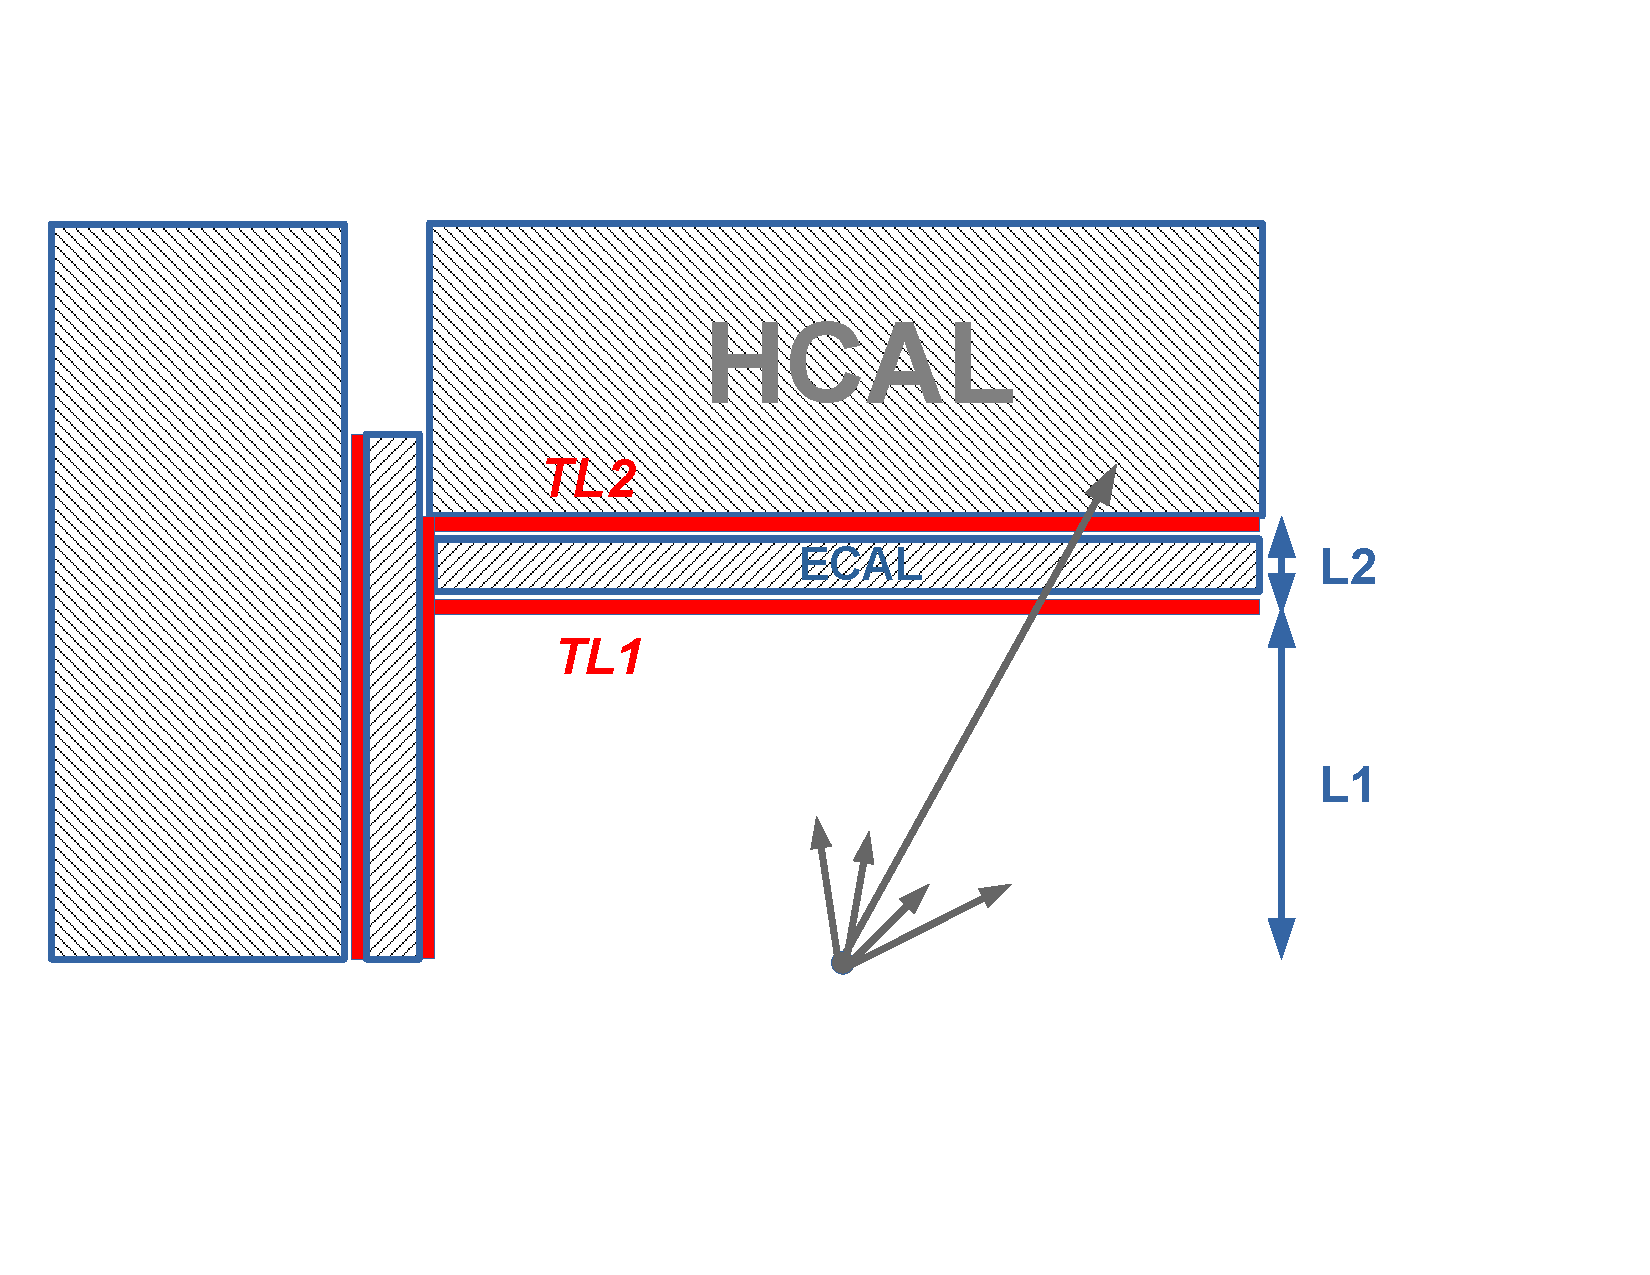
\includegraphics[width=0.8\textwidth]{timing_layer.pdf}\hfill
\end{center}
\caption{An example of positions of the thin timing layers for a generic detector. The thin timing layers  will enclose the electromagnetic calorimeter, allowing 
a reliable reconstruction of the  MIP signals with a timing resolution of the order of 10~ps.}
\label{fig:eff_rad}
\end{figure}


There are several reasons why the second timing layer (TL2) can be useful:

\begin{itemize}

\item
It can be used to measure the TOF between TL2 and TL1 for identification
of stable massive particles without known production vertex. This is especially important
for the BSM models predicting stable heavy particles
decaying close to the surface of the electromagnetic calorimeter.     

For a typical ECAL based on the silicon technology, the distance between TL2 and TL1 is  0.2 -- 0.4~m (depending on the calorimeter design).
It is not immediately obvious that such a small distance can be used for physics measurements. 
A particle traveling with the speed of light can cross the distance between TL1 and TL1 within $\sim 1$~ns.
As we will discuss later, this distance is sufficient to provide a large acceptance 
for heavy particle identification  assuming a 10 -- 20~ps detectors. 

\item
The second layer is  useful in the cases when a long-lived particle (neutral or charged) is produced without precise knowledge of the primary vertex (0,0,0)
due to the beam (or pileup) smearing. 

\item
It allows to correlate the hits with the first layer, and thus provides directionality of the hits. This feature can be useful to
match the hits with the calorimeter cells and to deal with back-scatter 
hits which are typically arriving from the hadronic calorimeter at later time. 

\item
It provides the redundancy for the calculation of TOF using the distance from the interaction point which can be determined using tracks.

\end{itemize}


The second layer of the timing detector can be justified if the recorded time difference between
the first and the last ECAL  
layers of the electromagnetic showers is not significantly different from that expected from a particle traveling with the speed of light.
If the travel time is significantly affected by large fluctuations caused by electromagnetic showers,    
second timing layer cannot effectively be used.

In order to verify this point, we used a full Geant4 (version 10.3)~\cite{Allison2016186} simulation 
of the SiFCC detector \cite{Chekanov:2016ppq} that allows to use the information of the ECAL hits.
This detector design has an ECAL built from a highly segmented silicon-tungsten cells with the transverse size of $2 \times 2$~cm.
The ECAL has 30 layers of tungsten pads with silicon readout,
corresponding to 35~X$_{0}$. The first 20 layers use tungsten of 3~mm thickness.
The last ten layers use tungsten layers of
twice the thickness, and thus have half the  sampling fraction.  
The distance between the centers of the last and first ECAL layer is about 240~mm.  

To verify that the time differences between the last and the first ECAL layer is close to the time
required for a particle that travels with the speed of light, and can be neglected for the timing layers that
have a timing resolution of the order of 1~ns, a sample of single pions ($\pi^\pm$) was created with 1 and 10~GeV momentum, respectively. The
pseudorapidity for all pions was $\eta=0$ (central region). 
The particles were reconstructed in the ECAL calorimeter,
and the time difference $\Delta T= T_{\mathrm{last}}-T_{\mathrm{first}}$ of the hits between the last and first ECAL layers was calculated.
Only the hits arriving first in time were considered since the electronics typically register\footnote{The Monte Carlo studies used in this paper does not include
simulations of calorimeter electronics.} the fastest hits (while slower hits can be saved in pipeline buffers).

Figure~\ref{fig:timediff} shows the time distribution of first arriving hits 
for 1 and 10 GeV pions. It can be seen that the peak positions of the distributions are smaller
than 1~ns, as expected for the distance of about 20~cm between  the centers of the last and first ECAL layers.
Therefore, the hits registered by TL1 and TL2 will be simultaneous for the
standard 1~ns resolution readout. They will be fully correlated in time, and are identified as a single crossing particle.

If a resolution of the timing layer is of the order of 10 -- 20~ps, a physics measurement of TOF would be possible.
To check this, 
Figure~\ref{fig:timediff} shows the hit distribution for (anti)deuterons, denoted as $d^{\pm}$. 
The distributions are significantly different from the $\pi^{\pm}$ case. According to the simulation, the 1~GeV
(anti)deuterons should be measured on average with the time delay of 0.7 -- 1.4~ns between the last and first layers.
The value of 0.7~ns was estimated from the mean position of the Landau distribution used to fit the $d^{\pm}$ 
curve presented in Figure~\ref{fig:timediff}(a),
while 1.4~ns was obtained from the mean of this distribution. Even for the most conservative 0.7~ns value, there is an indication that 1~GeV
deuterons can be separated from pions that have 0.5~ns time difference. Such a separation can be observed when using a tens-of-picosecond detector.
For the 10~GeV particles presented in Figure~\ref{fig:timediff}(b), no separation between $d^{\pm}$ and $\pi^{\pm}$ can be observed.

In summary, we have illustrated that a typical difference between TL2 and TL1 (which is approximated by the difference
between the last and first ECAL layer) is sufficient for particle identification using the TOF.
As an example, a $d^{\pm}$ can be identified and separated from pions for the momentum less than 1~GeV.
This means that  particles heavier than deuterons should be identified for a momentum larger than 1~GeV.
In the following, we will abstract from the Geant4 simulations and calculate the kinematic regions  where the identification of heavy stable 
particles using timing layers is possible.
 

\begin{figure}
\begin{center}
   \subfigure[] { 
   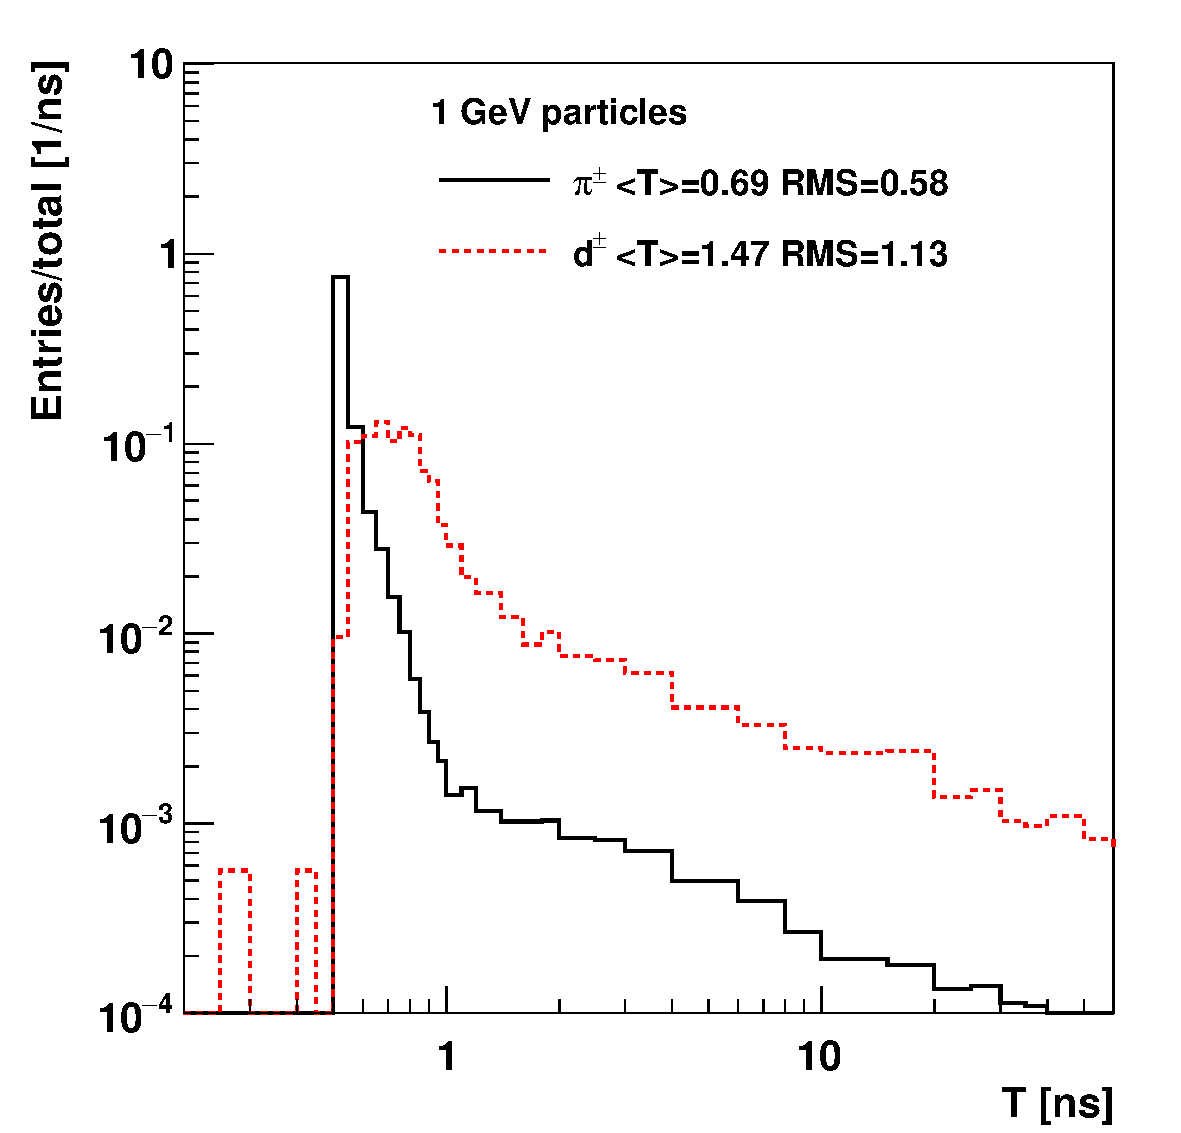
\includegraphics[width=0.45\textwidth]{timeECAL_2layers_1gev1.pdf}\hfill
   }
   \subfigure[] { 
   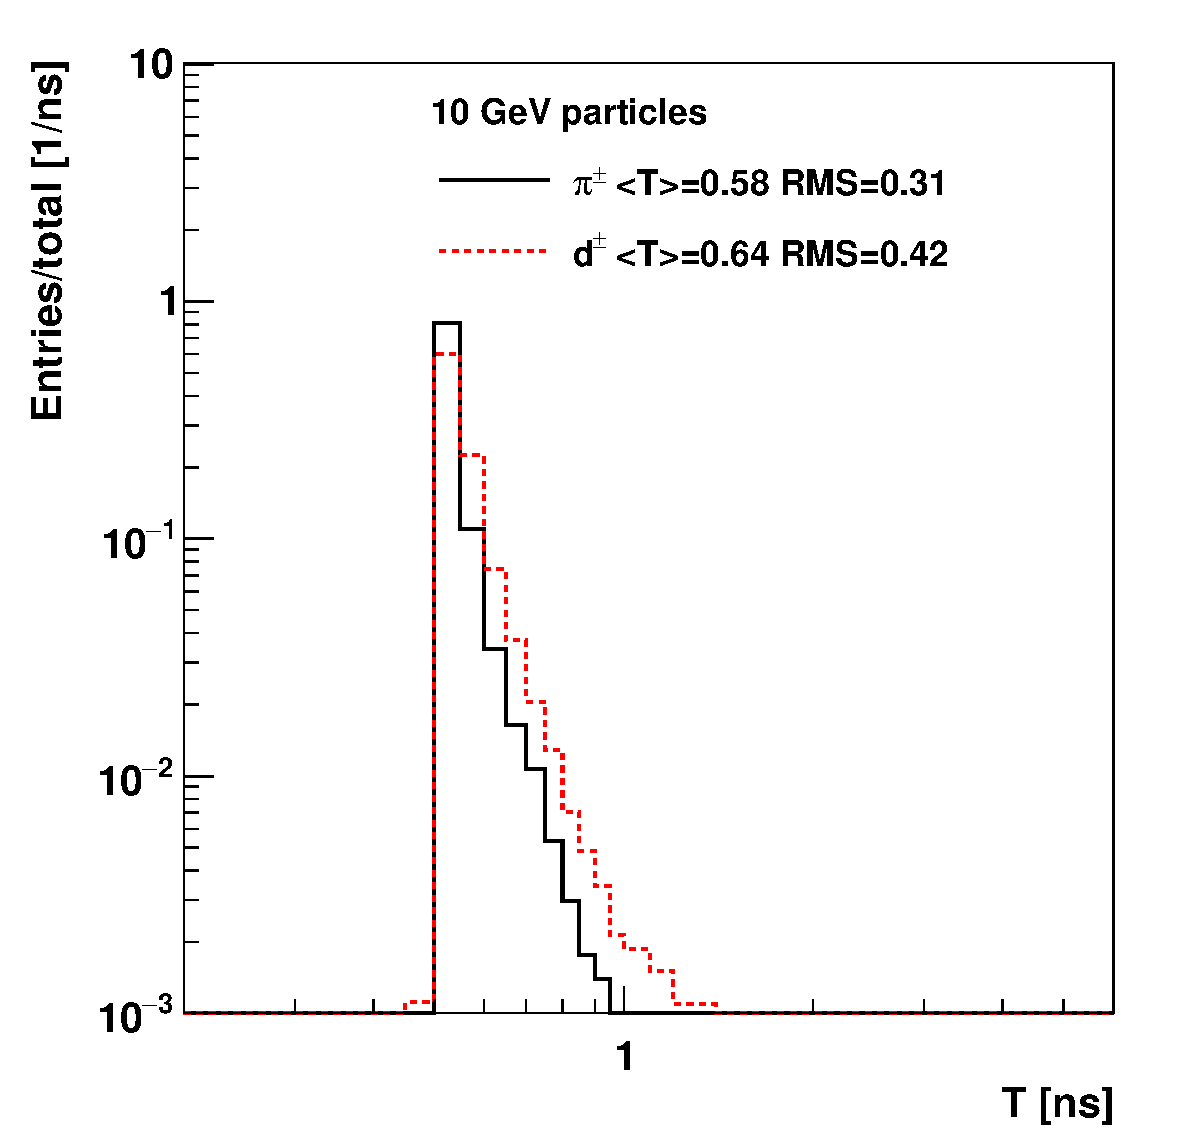
\includegraphics[width=0.45\textwidth]{timeECAL_2layers_10gev1.pdf}\hfill
   }
\end{center}
\caption{The difference between time of hits between the last and first layer of ECAL for single pions and deuterons  with a transverse momentum of (a) 1~GeV  and (b) 10 GeV. 
Only first (fastest) hits were considered to calculate the difference in TOF. }
\label{fig:timediff}
\end{figure}



\clearpage 
%%%%%%%%%%%%%%%%%%%%%%%%%%%%%%%%%%%%%%%%%%%%%%%%%%%%%%%%%%%%%%%%%%

%%%%%%%%%%%%%% sections 
\section{Timing layers for single particles}

Now we discuss the kinematic regions  relevant for  TOF measurements of SM and BSM particles. Instead of the full {\sc geant}4 simulations, we will
use a semi-analytic approach.  
 
To estimate the separation power between different mass hypotheses, we calculate the mass and momentum for which one can achieve a separation 
 significance higher than $3\sigma$ (or p-value$<0.3$\%). 
If there are two particles with mass $m$ and a reference (fixed) mass $m_F$, respectively, the $3\sigma$ separation can be 
achieved for this condition~\cite{Cerri:2018rkm}:
\begin{equation}
\frac{L}{c \sigma_{\textsc{TOF}}}\left|\sqrt{1+\frac{m^2}{p^2}} - \sqrt{1+\frac{m_F^2}{p^2}}\right| > 3
\label{eqTOF}
\end{equation}
where $p$ is the momentum of a particle with mass $m$, $L$  is the length of the particle's trajectory, 
and $\sigma_{TOF}$ is the
resolution  of the timing layer that measures the TOF.

Figure~\ref{fig:singleparticles} shows the $3\sigma$ separation from the pion
mass hypothesis ($m_F=m_{\pi}$) using the procedure discussed  in~\cite{Cerri:2018rkm}. The 
calculations are performed for several values of resolution of the timing layer, ranging from 10~ps to 1~ns,
as a function of $L$ and $p$. For a 20~ps detector and a typical travel 
distance $L\sim 1.5-2$~m from the production vertex to the ECAL, neutrons and protons can be separated from the pion hypothesis up to $p \approx 7$~GeV. 
The separation of kaons from pions can be performed up to 3~GeV.
This momentum range should be sufficient for a reliable particle 
identification in a momentum range adequate for some physics studies focused on
single-particle reconstruction (such as B-meson physics).
This can also be used for jets that are dominated
by particles in this momentum range.
For a detector  with 1~ns resolution, the separation can only be possible  up to  300 -- 500~MeV. This is smaller than the 
minimum particle momentum of $\approx$0.5~GeV considered for high-energy proton colliders.
Therefore, a timing layer with 1~ns resolution cannot be used for particle identification in such experiments.

\begin{figure}
\begin{center}
   \subfigure[Neutrons] {
   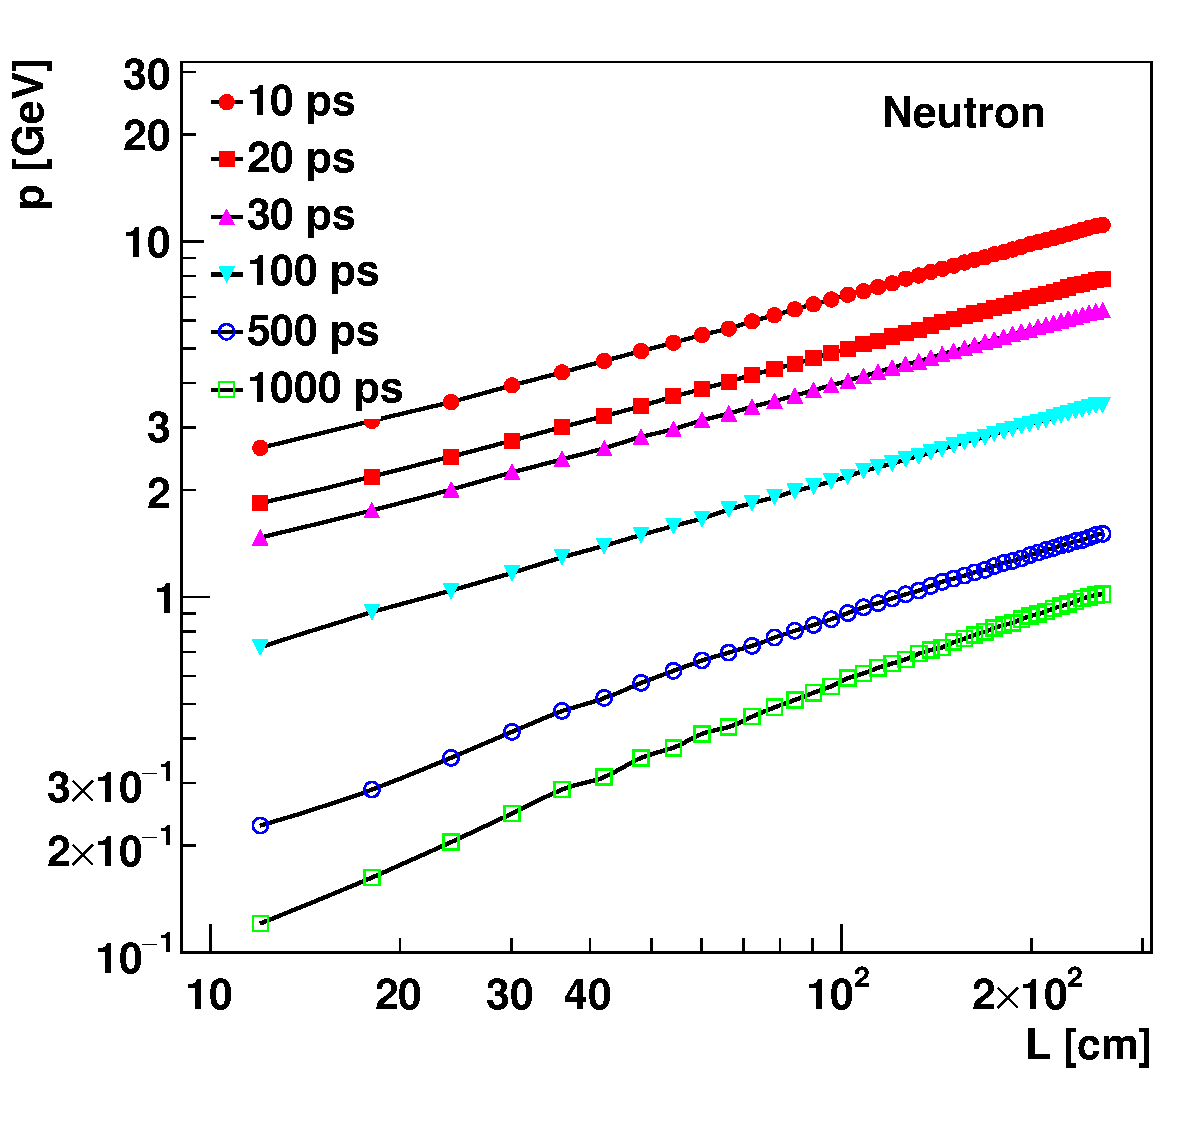
\includegraphics[width=0.45\textwidth]{time_flight_length_neutron.pdf}
   }
      \subfigure[$K$-mesons] {
   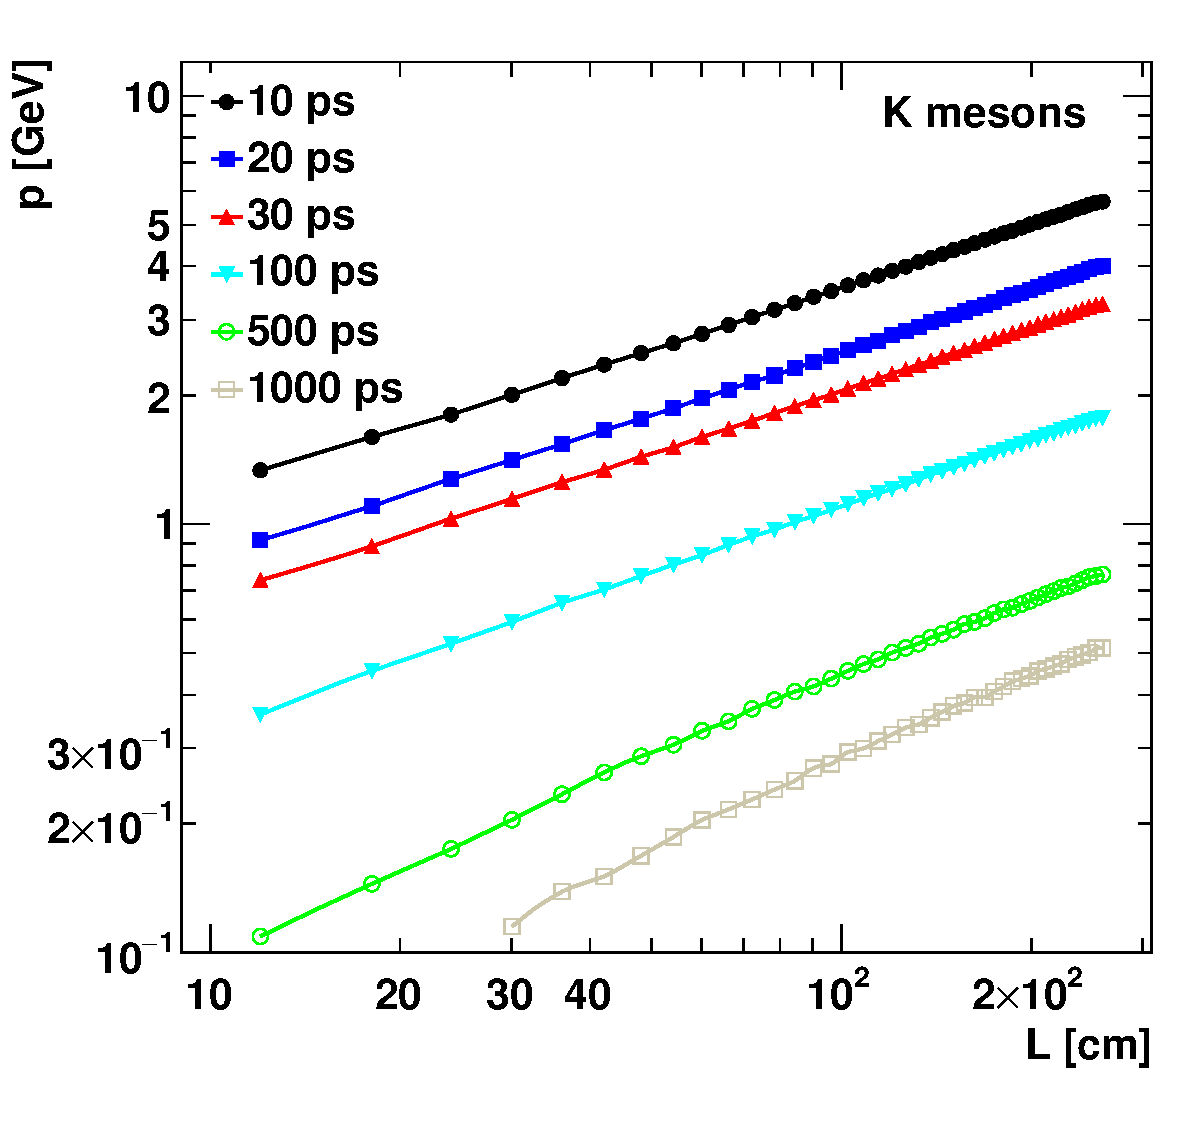
\includegraphics[width=0.45\textwidth]{time_flight_length_kion.pdf}\hfill
   }
\end{center}
\caption{
The $3\sigma$ separation from the pion-mass hypothesis for (a) neutrons and (b) kaons as a function of the length of the particle's trajectory $L$ 
and the momentum $p$. The lines show extrapolated results between the calculations indicated by the symbols.  
}
\label{fig:singleparticles}
\end{figure}


\begin{figure}
\begin{center}
   \subfigure[for $L=2$~m] {
   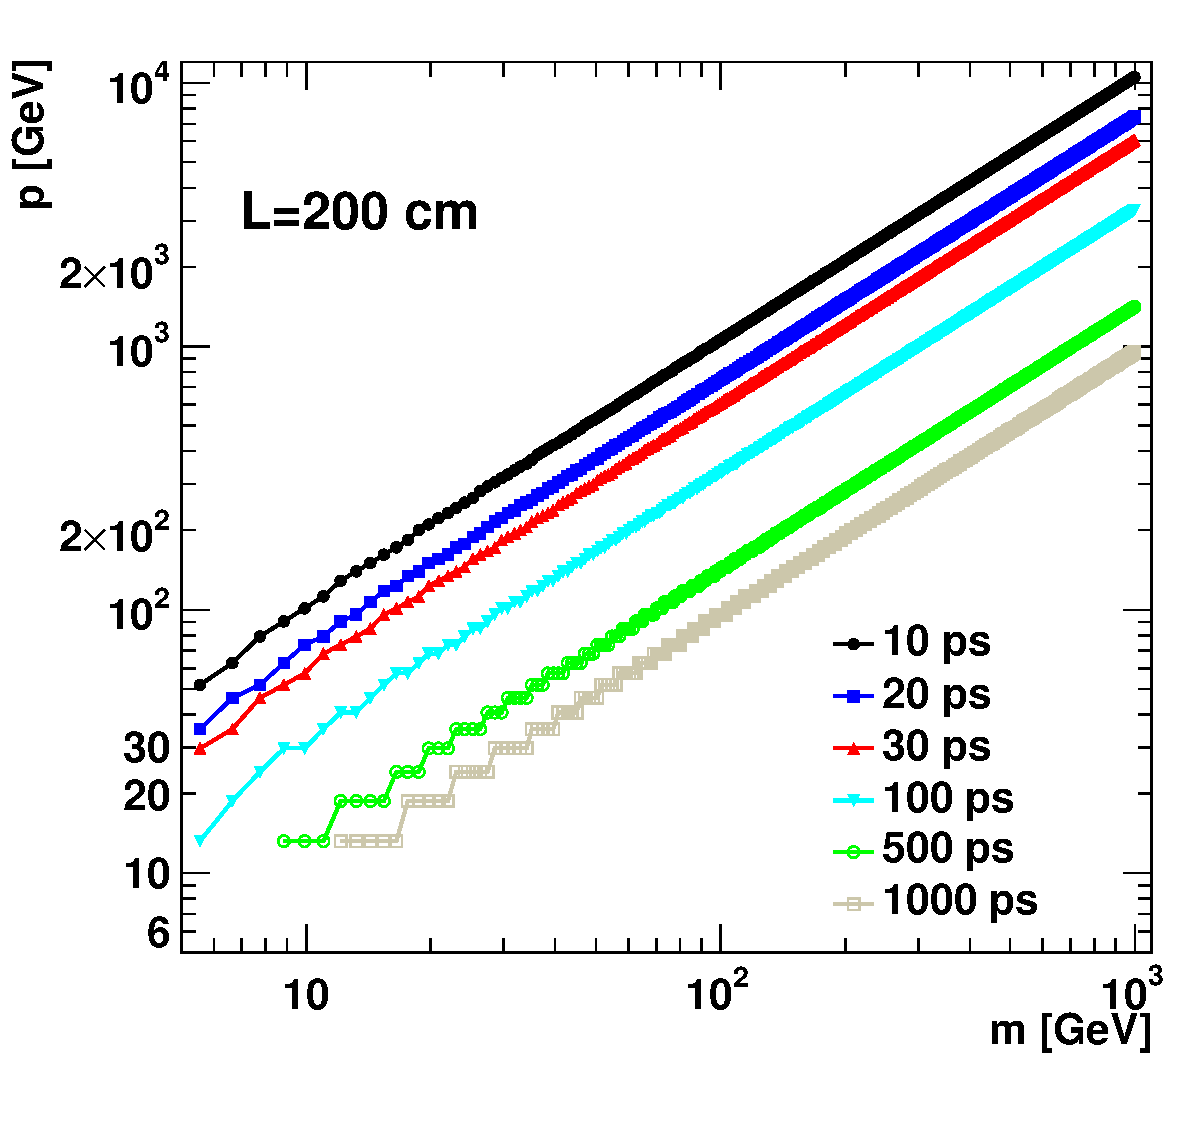
\includegraphics[width=0.45\textwidth]{time_flight_200.pdf}
   }
   \subfigure[for $L=0.2$~m] {
   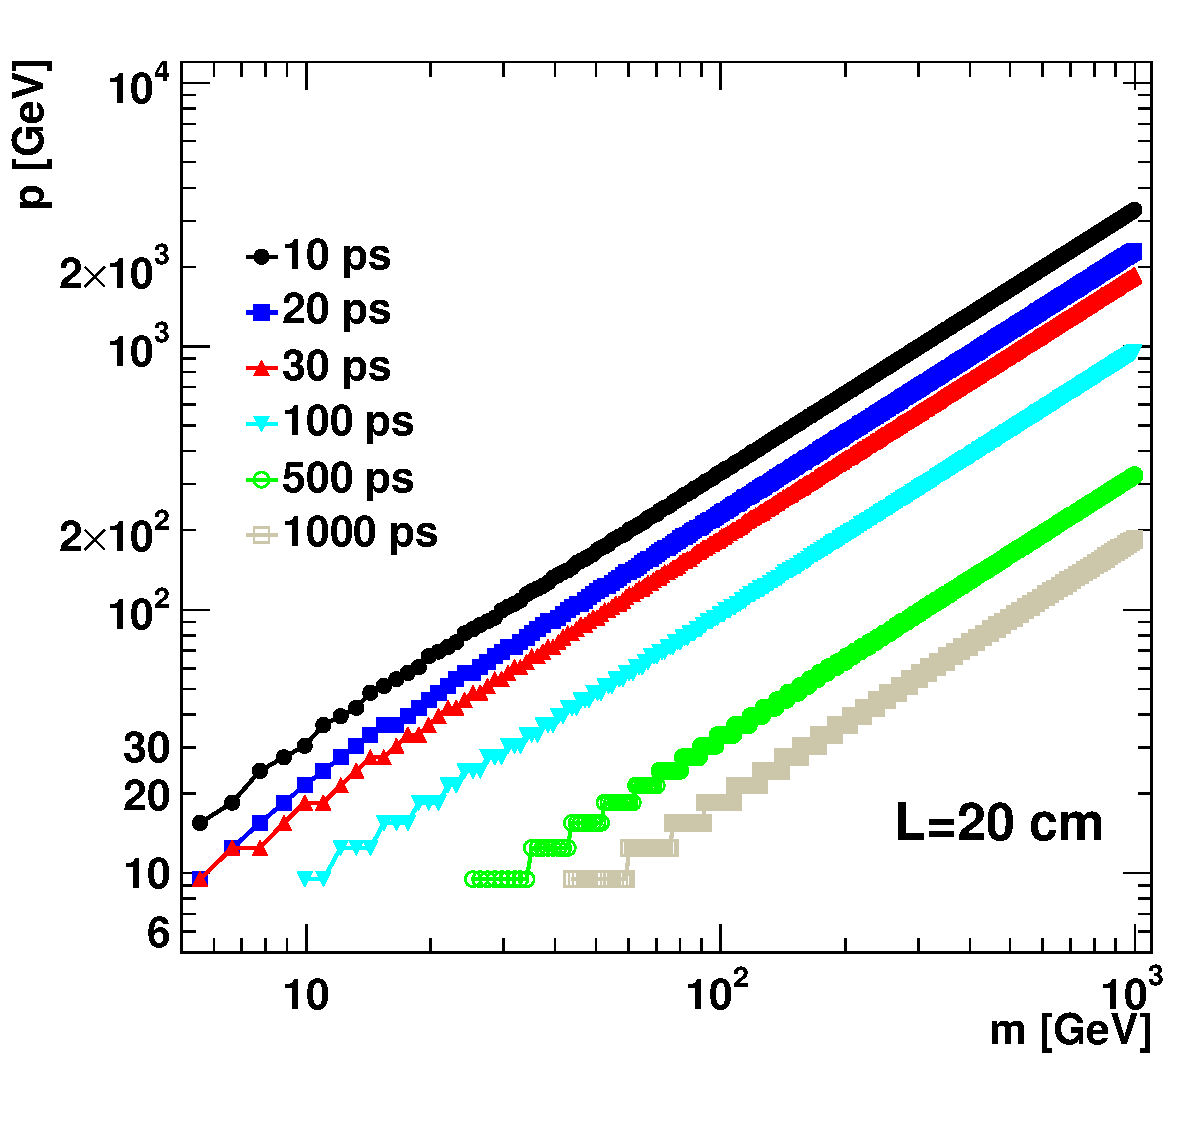
\includegraphics[width=0.45\textwidth]{time_flight_20.pdf}\hfill
   }
\end{center}
\caption{
The $3\sigma$ separation between heavy particles and $\alpha$ particles assuming timing layers with different resolutions for TOF, and using (a) $L=2$~m and (b) $L=0.2$~m.
The first value of $L$ is the typical distance
from the interaction vertex to the first layer TL1, while the second value is the typical  distance
between the two timing layers enclosing an ECAL based on the silicon technology.
}
\label{fig:signgleBSM}
\end{figure}

Having discussed the rather classical cases of discriminating  neutrons, protons and kaons from the pion hypothesis,
let us turn to the BSM searches for heavy particles.
The largest SM  backgrounds for light BSM  particles are primary protons and neutrons.
Other stable particles that can be produced by secondary interactions in the 
detector material or the beam pipe are deuterons and $\alpha$ particles. 
Although the $\alpha$ particle rate is  low since they stop easily in detector material,
it may still represent background for rare BSM particle searches.  
Therefore, we choose  $m_F=m_{\alpha}\simeq 3.73$~GeV  as reference\footnote{We clarify that the choice of $\alpha$ particles as the reference mass is
arbitrary and is only motivated by our attempt to check the $3\sigma$ separation in the momentum range $p<10$~GeV.} in  Eq.~\ref{eqTOF}, and evaluate the
$3\sigma$ separation for a wide range of masses and momenta above 4~GeV.
For many planned experiments the distance between the $pp$ collision point and the first layer of the ECAL is 
$1.5-2.5$~m. Therefore we use $L=2$~m and consider 0.2~m as the separation between the TL2 and TL1 timing layers.

Figure~\ref{fig:signgleBSM} shows the discrimination power for different choices of the timing layer resolution
and the distance $L$ (see Fig.~\ref{fig:eff_rad}).
For $L=2$~m, a stable heavy particle of mass 100~GeV can be discriminated for momentum up to 
700~GeV assuming a 20-ps timing layer,
but only up to 50~GeV using the standard 1~ns resolution.

When  TOF is measured between the layers TL1 and TL2, and assuming a spatial match of the hits, the knowledge of the interaction vertex is not required.
This type of measurement can be beneficial for neutral particles in events with large pile-up (multiple $pp$ collisions).
The identification power when $L=0.2$~m, i.e. the distance between TL2 and TL1, is shown in Fig.~\ref{fig:signgleBSM}(b).
For a stable particle with mass 100~GeV, the identification is possible up to about 200~GeV in momentum. The standard calorimeter with
1~ns resolution can only perform the identification up to $20$~GeV. 


\section{Showcase for the Dark QCD model}
\label{darksec}

The arguments discussed above can be illustrated using concrete BSM physics scenarios.
We will consider the ``dark'' QCD model~\cite{Bai:2013xga,Schwaller:2015gea}, which predicts 
the existence of ``emerging'' jets 
that are created in the decays of new long-lived neutral 
particles (dark hadrons), produced in a parton-shower process by dark QCD.
The process includes  two mediators of mass $M_X$ which 
decay promptly to a SM quark and a dark quark. 
The final-state signature consists of four jets with high transverse momenta, with two  
 emerging jets originating from the dark quarks.  

Searches for emerging jets have been performed in $pp$ collisions~\cite{Sirunyan:2018njd} 
by the CMS Collaboration. Such jets contain many displaced
 vertices and multiple tracks with large impact parameters, arising from the decays of the dark pions produced in the dark parton shower.
 Assuming that the mass of the dark pion is 5~GeV,  the signal acceptance using this approach does not exceed 40\% at large masses of the mediators
(see Fig.~4 of~\cite{Sirunyan:2018njd}).
The decay length of the dark pion defines the distance from the $pp$ interaction vertex 
to the point where the jet emerges. 

Alternatively, emerging jets can be reconstructed using calorimeters with high-resolution timing. This method is expected
to have advantages over the track-based method 
for the measurement of dark pions with a large decay length, i.e. in the situations where the tracker has a low
efficiency and resolution since only a few outer layers can be used for track reconstruction.
It was also pointed out~\cite{Schwaller:2015gea} that the emerging jets may have a significant fraction of neutral particles and the reconstruction
using charged tracks can have a low acceptance.

To estimate the performance of the timing layers in reconstructing emerging jets,
we use the same Monte Carlo generator settings as for Ref.~\cite{Sirunyan:2018njd}. 
The $pp$ collision event samples  were  generated with the ``hidden valley'' model framework in {\sc pythia} 8.2 assuming a centre-of-mass energy 
 of 13~TeV and a dark pion mass of 5~GeV. The samples were created for different values of the decay distance $c\tau$ of the dark pions.  
The  mass $M_X$ of the mediator was also varied. 

To calculate the detector acceptance, the semi-analytical formalism based on Eq.~\ref{eqTOF} is used. In this relation $L=c\tau$ is the distance traveled
by the dark pion with mass $m$ before it decays to the emerging jet.  
We assume that such emerging jets travel to the surface of the timing layer with speed of light for all values of $m$.
This is expected since the emerging jets consist of light stable SM particles (mostly photons and pions).
  
For the timing layers, the signature of emerging jets is a time delay compared to the other SM jets. The  production vertex
cannot be observed by the timing layers if such jets emerge before TL1.
After events are generated, the weighted averages of the decay distances of all particles that originate from
the dark pions, using the particle momentum as the weight, were  calculated. This decay distance is used
to approximate the decay length, without applying a jet reconstruction algorithm.  
The  calculation for the $3\sigma$ separation assumes $m_F=m_{\alpha}\simeq 3.73$~GeV although this choice can be arbitrary.
This value of $m_F$ is used to give a conservative\footnote{One can argue that the SM jets mainly consist of light-flavour hadrons and photons, 
therefore, $m_F$ should be significantly lower.} estimate of the arrival time of the emerging SM jets.

The acceptance of the emerging jets was calculated as the fraction of  events that pass the 
Eq.~\ref{eqTOF} condition  with the parameters discussed earlier. 
 Figure~\ref{fig:efficiency_med} shows the acceptance as a function of the mediator mass $M_X$ and the decay distance
of the dark pions. This acceptance can be compared to the acceptance based on tracks~\cite{Sirunyan:2018njd}. 
The acceptance based on the TOF is significantly larger for low $M_X$ and large $L=c\tau$ of the dark pions.  
The acceptance is larger for the timing layers with a resolution better than 100~ps, as compared to the standard 1~ns resolution. 

We are interested in the acceptance  for dark pions  as a function of their mass
and lifetime assuming a fixed mass $M_X$ of the mediator. We  consider the HE-LHC environment 
with $pp$ collisions at a centre-of-mass energy of 27~TeV.    
The Monte Carlo generator settings for the signal model were similar
to those discussed in~\cite{Sirunyan:2018njd,prive}.
The mediator mass was set to 10~TeV, while the mass of the dark pion was varied in the range between 5~GeV and 1~TeV.
The dark pion decay length, $c\tau$,  was varied between 1~mm and 1000~mm, independent of its mass. Other parameters
were also appropriately modified to allow  sufficient phase space for the dark meson production.
The mass of the dark pion is assumed to be one half the mass of the dark quark. The mass of the dark
$\rho$ is four times the dark pion mass. The width of the
mediator particle is assumed to be small compared to the detector mass resolution.

As before, the acceptance for the emerging jets based on timing was calculated as the fraction of events that pass the 
Eq.~\ref{eqTOF} condition. Figure~\ref{fig:efficiency} shows the efficiency
as a function of $c\tau$ and the dark pion mass. It can be seen that a detector with the standard 1~ns resolution does
not have acceptance for the dark meson measurements. The acceptance is significantly larger when the timing layers 
 have a resolution better than 100~ps.
The acceptance is low for small $c\tau$ or small masses, which is the expected feature of the timing measurement.
The timing layers with 20~ps resolution have 100\% acceptance for large values of $c\tau$ and dark-meson masses.
The acceptance as a function of the particle velocity when using 20~ps and 1~ns resolution 
is shown in \ref{appendix}.

Note that these results are relatively general since they are formulated in terms of masses and decay lengths,  
i.e. independent of the position of the timing layers and other details relevant to 
the detector geometry.


\begin{figure}
\begin{center}
   \subfigure[10 ps] {
   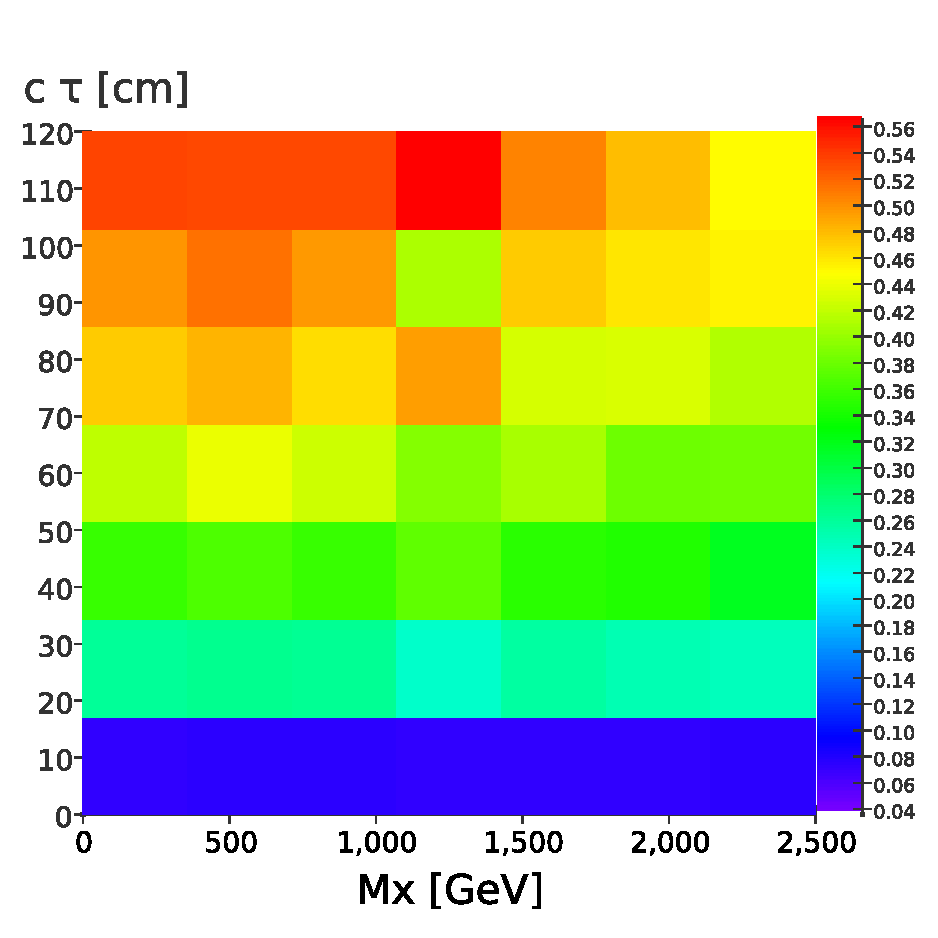
\includegraphics[width=0.4\textwidth]{effic10a_med.pdf}
   }
   \subfigure[20 ps] {
   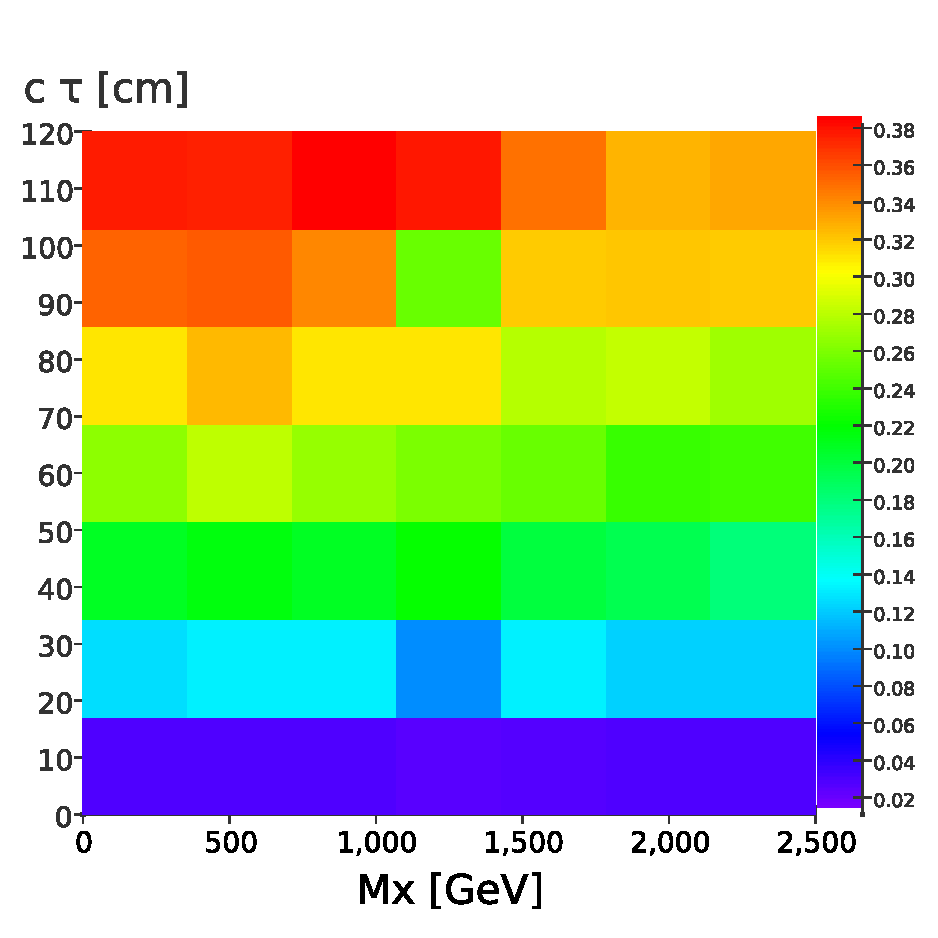
\includegraphics[width=0.4\textwidth]{effic20a_med.pdf}\hfill
   }

   \subfigure[30 ps] {
   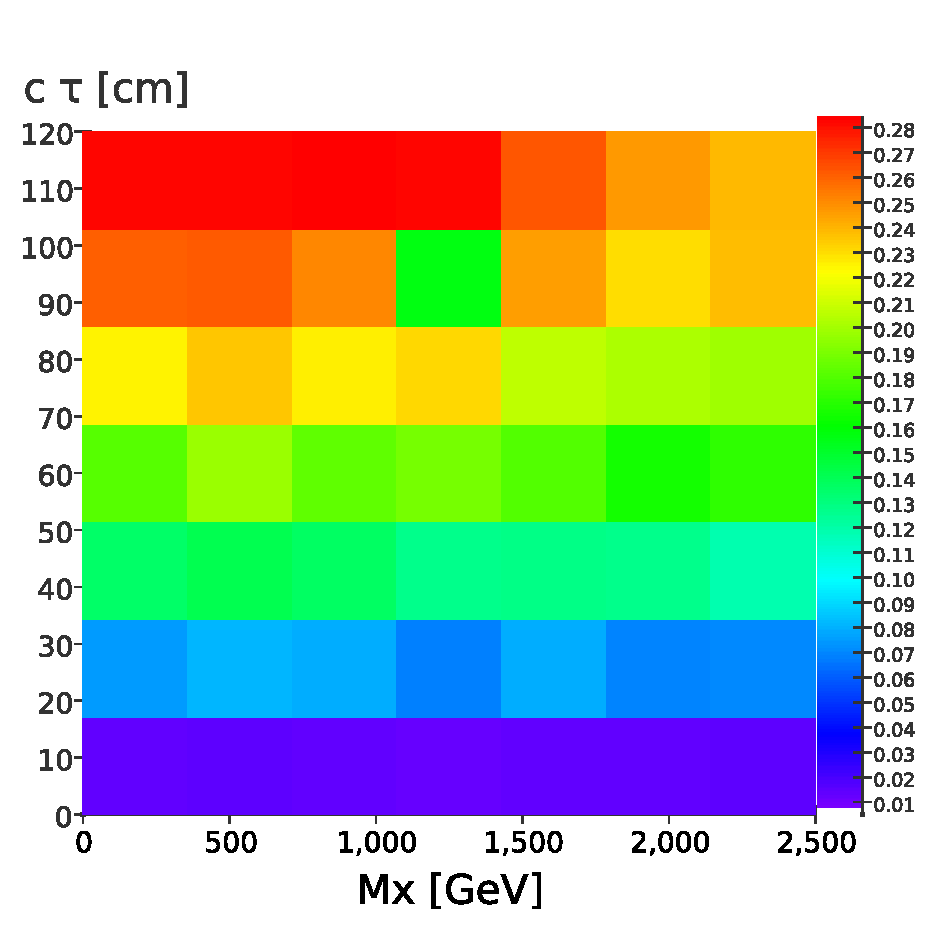
\includegraphics[width=0.4\textwidth]{effic30a_med.pdf}
   }
   \subfigure[100 ps] {
   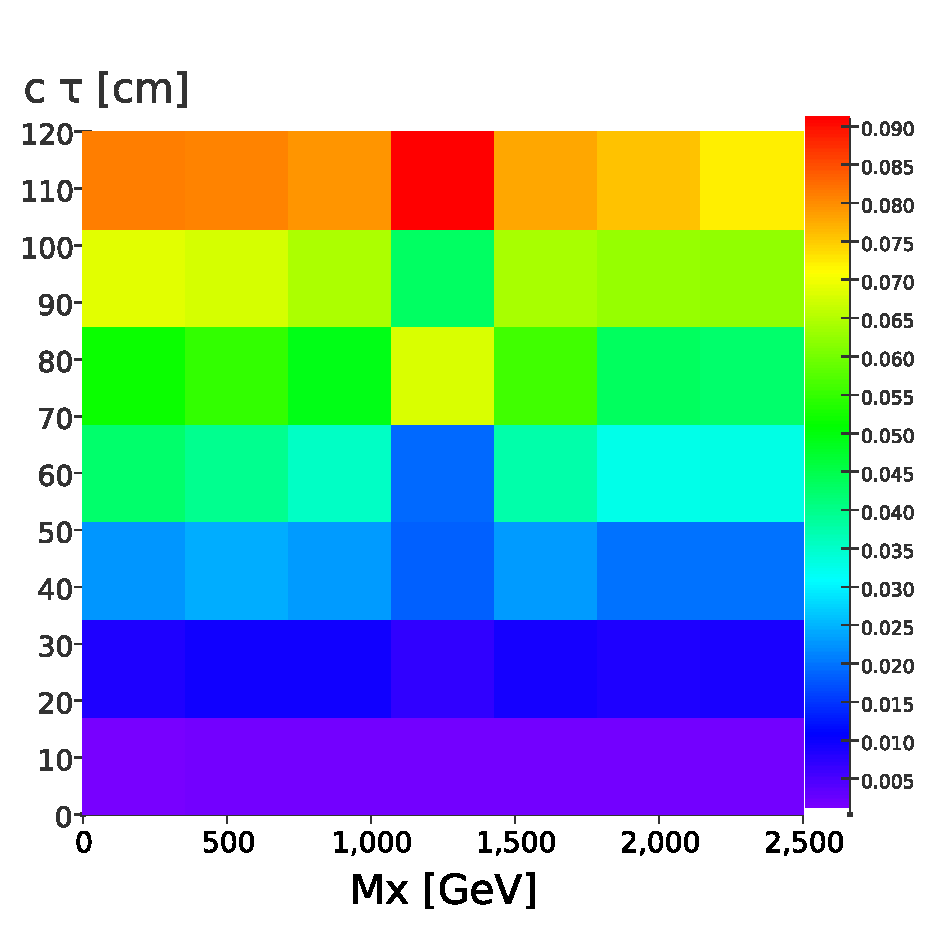
\includegraphics[width=0.4\textwidth]{effic100a_med.pdf}\hfill
   }

   \subfigure[500 ps] {
   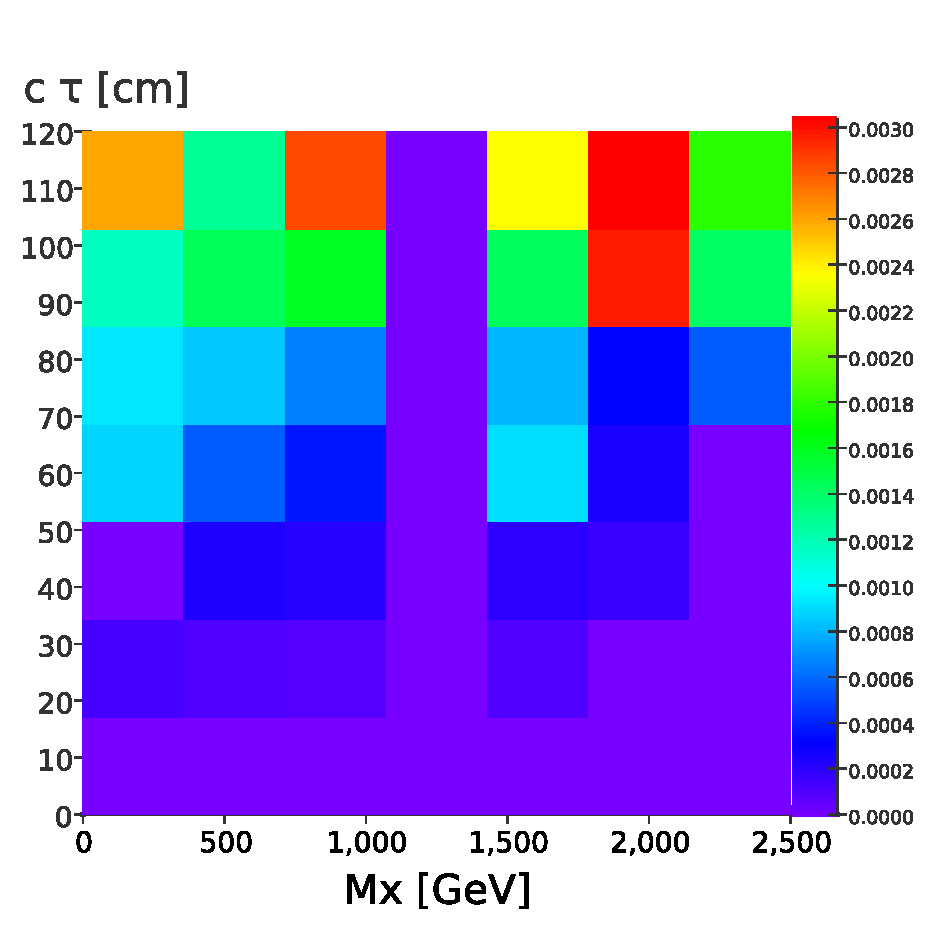
\includegraphics[width=0.4\textwidth]{effic500a_med.pdf}
   }
   \subfigure[1000 ps] {
   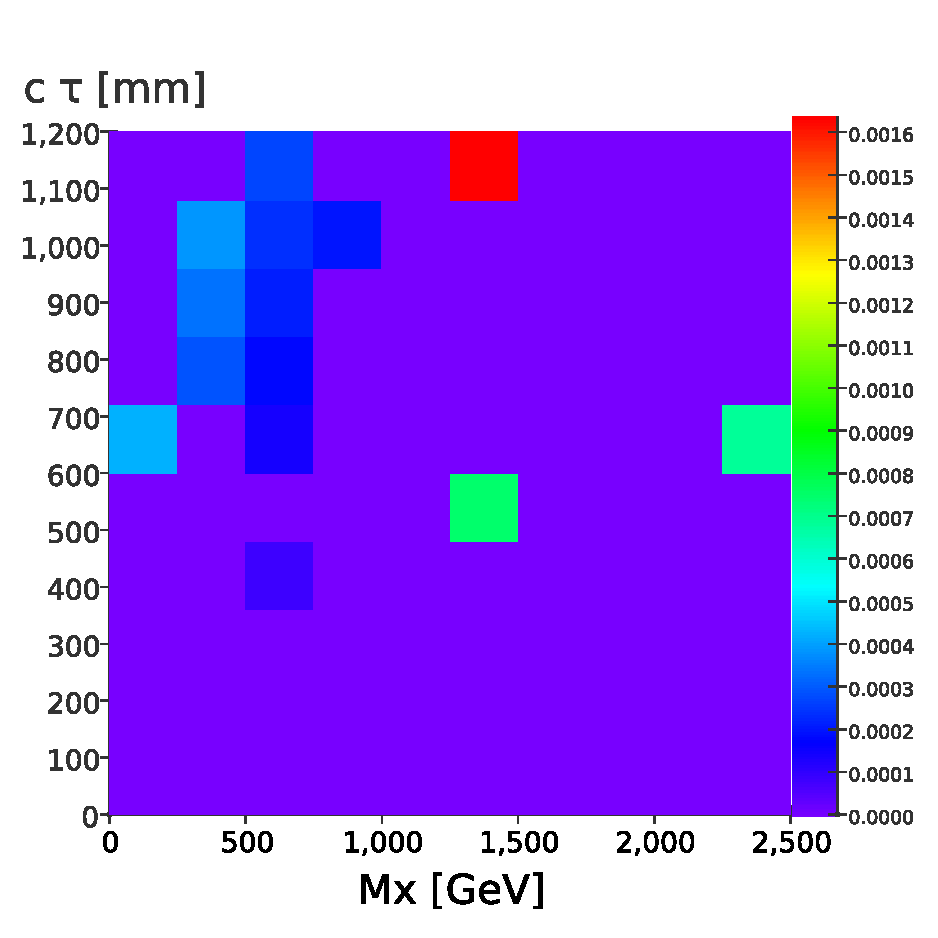
\includegraphics[width=0.4\textwidth]{effic1000a_med.pdf}\hfill
   }

\end{center}
\caption{
The acceptance for emerging jets using timing layers with different timing resolutions as
a function of the mediator mass $M_X$ and the $c\tau$ of the dark pions with mass of 5~GeV.
The {\sc pythia}8 simulations were performed
for $pp$ collisions at $\sqrt{s}=13$~TeV. 
}
\label{fig:efficiency_med}
\end{figure}

\begin{figure}
\begin{center}
   \subfigure[10 ps] {
   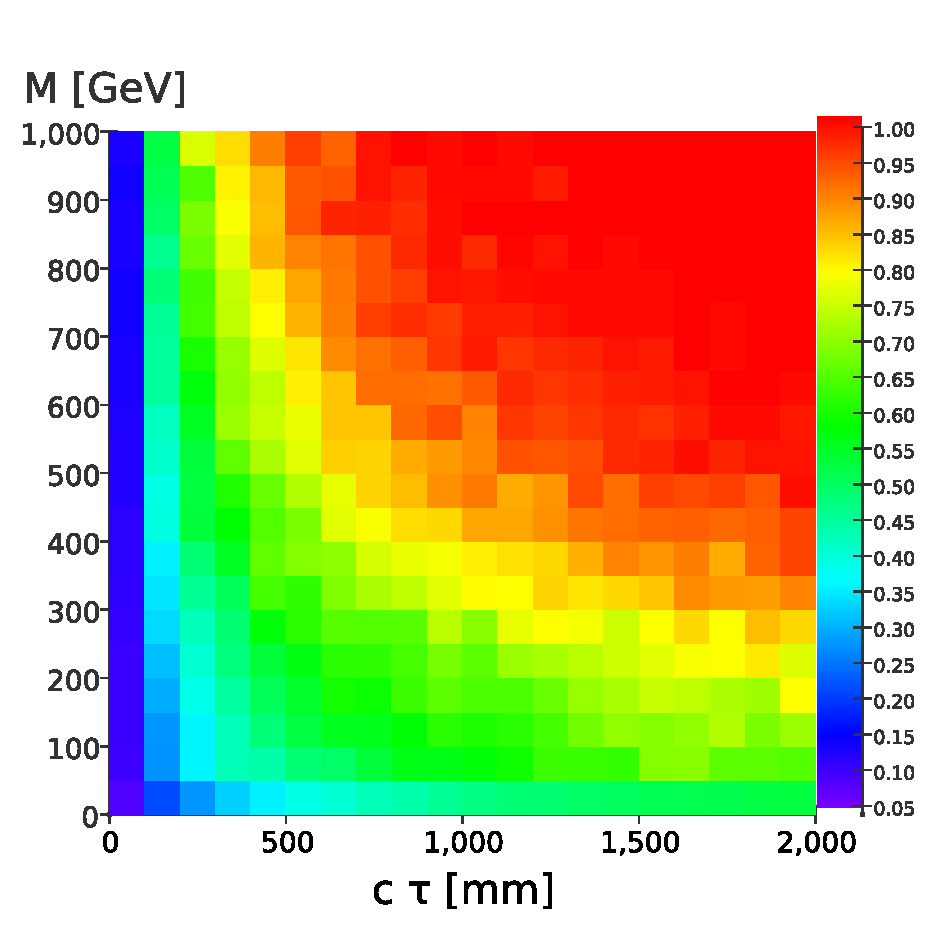
\includegraphics[width=0.4\textwidth]{effic10a.pdf}
   }
   \subfigure[20 ps] {
   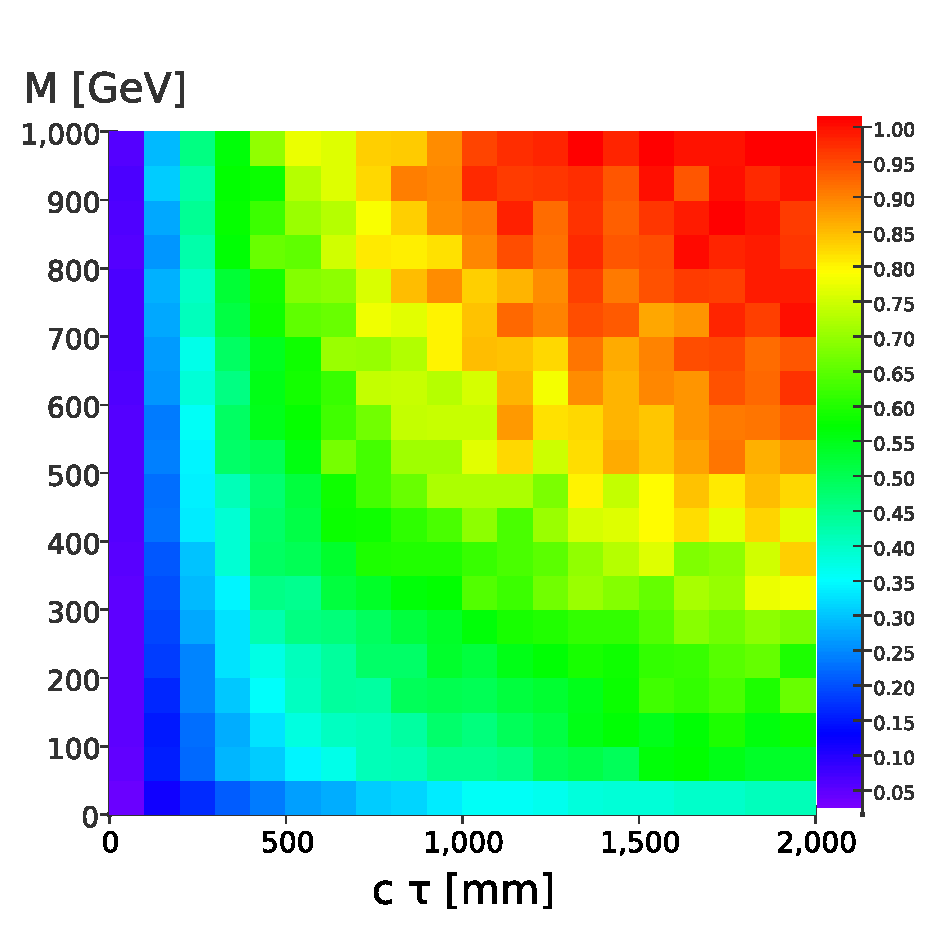
\includegraphics[width=0.4\textwidth]{effic20a.pdf}\hfill
   }

   \subfigure[30 ps] {
   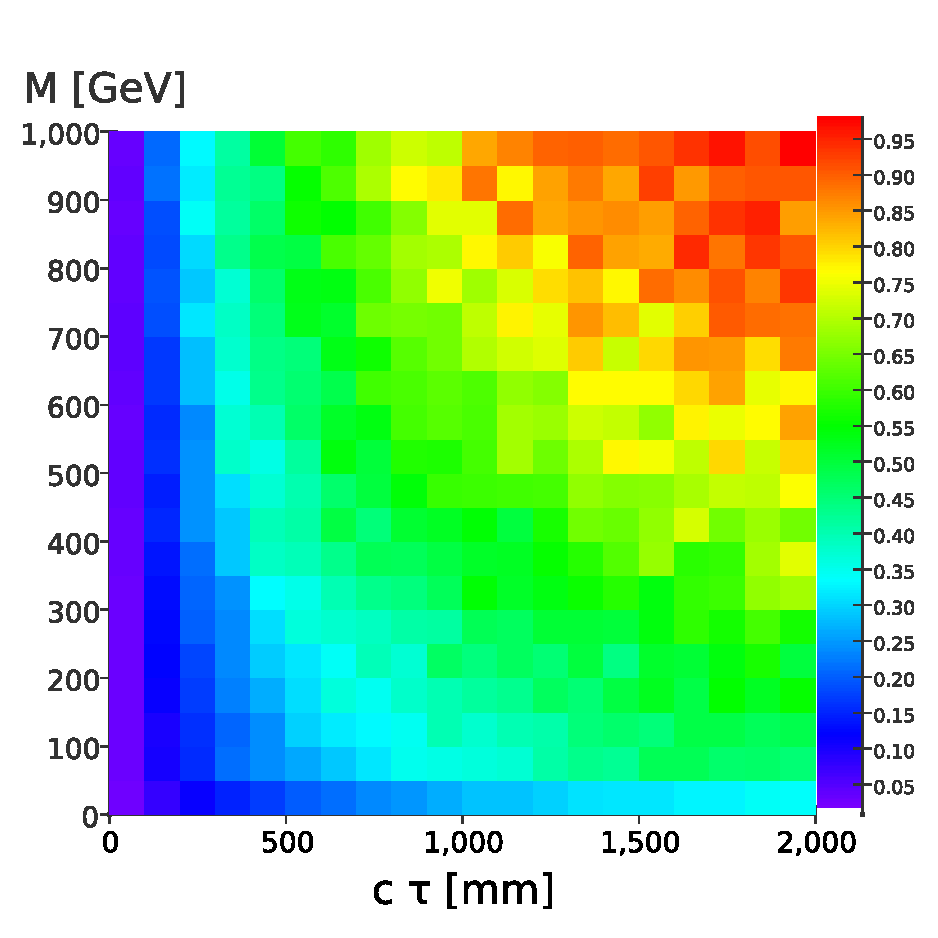
\includegraphics[width=0.4\textwidth]{effic30a.pdf}
   }
   \subfigure[100 ps] {
   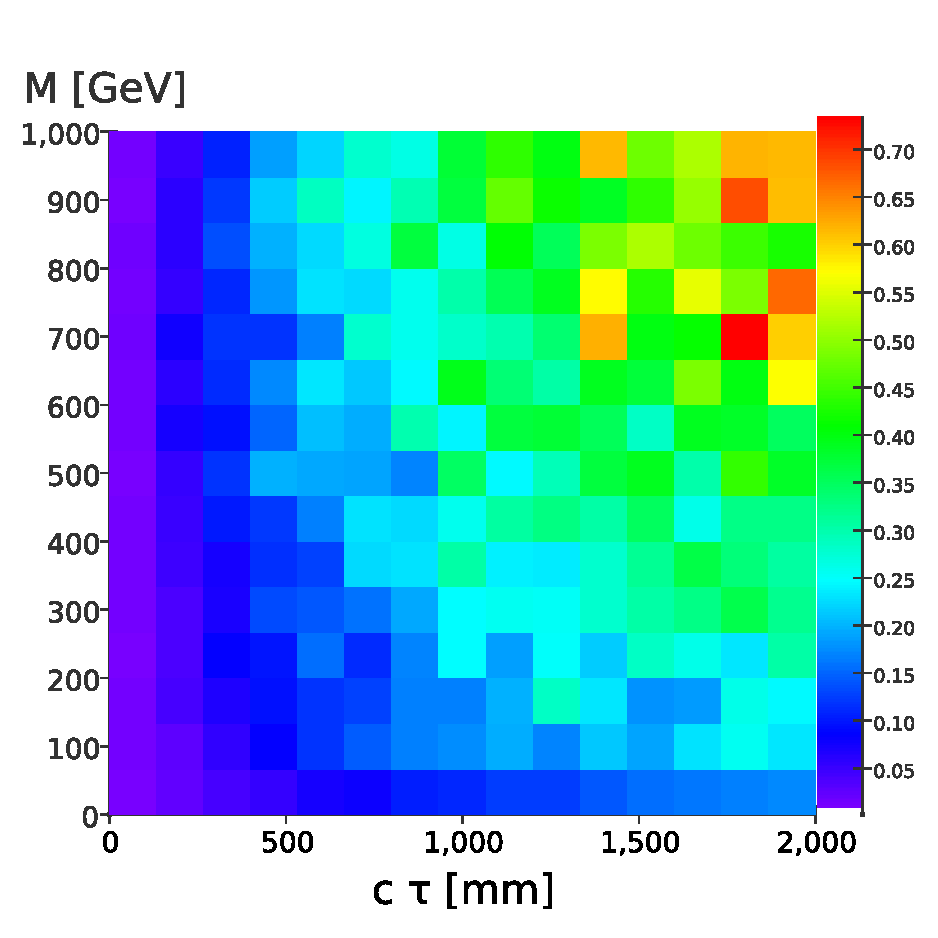
\includegraphics[width=0.4\textwidth]{effic100a.pdf}\hfill
   }

   \subfigure[500 ps] {
   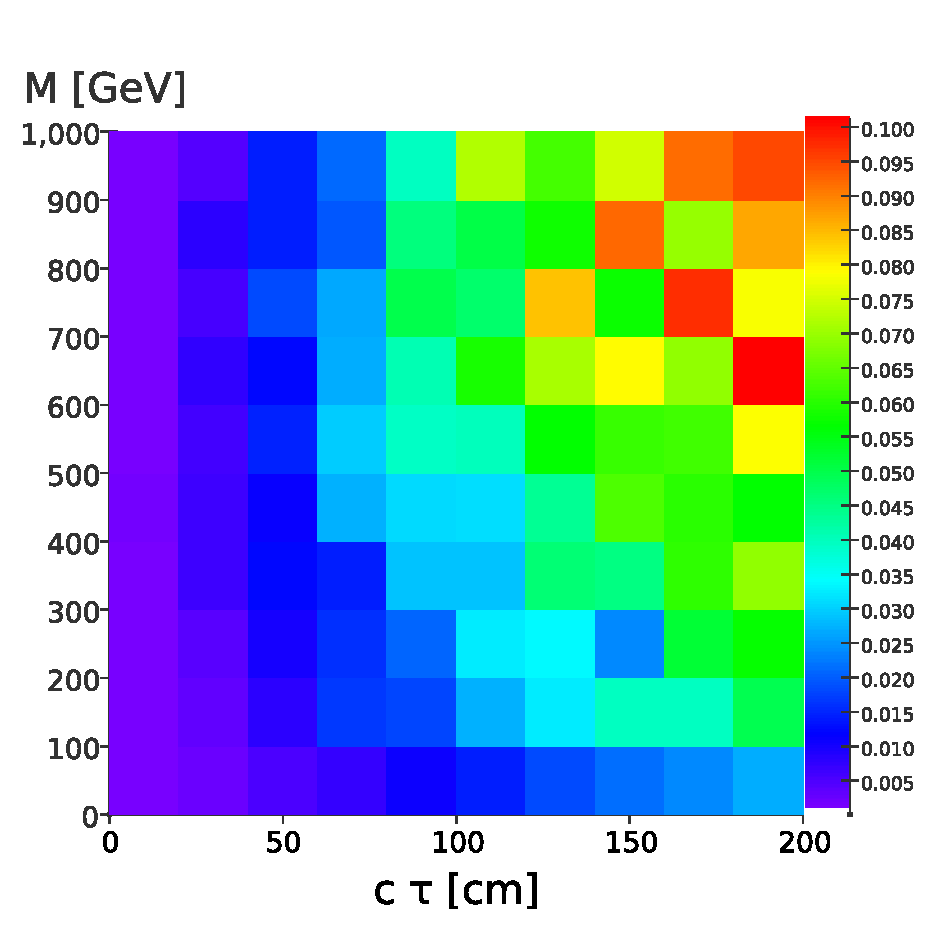
\includegraphics[width=0.4\textwidth]{effic500a.pdf}
   }
   \subfigure[1000 ps] {
   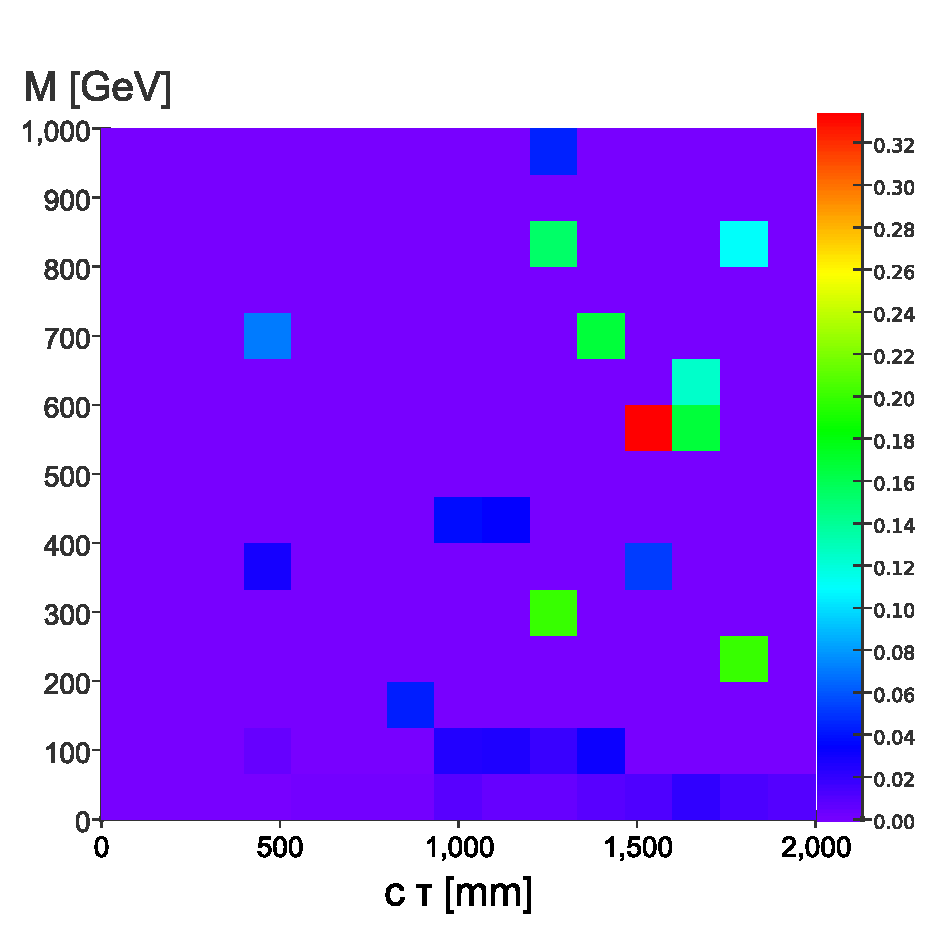
\includegraphics[width=0.4\textwidth]{effic1000a.pdf}\hfill 
   }

\end{center}
\caption{
The acceptance for emerging jets using timing layers with different timing resolutions as
a function of the dark pion mass and $c\tau$. The mediator mass was fixed at $M_X = 10$~TeV. The {\sc pythia}8 simulations were performed 
for $pp$ collisions at $\sqrt{s}=27$~TeV. 
}
\label{fig:efficiency}
\end{figure}



%%\section{Timing layers for ee experiments}

%%%%%%%%%%%%%%% commented out 
%\end{comment}


%\section{Timing layers for FCC and jets}

%%%%%%%%%%%%%%% commented out 
%\end{comment}




\section{Summary}

This paper discusses the benefits of the timing layers positioned in front of the hadronic calorimeters.
Using the full Geant4 simulations and a semi-analytic approach,
the figures of merits for identification of single particles
using timing layers with resolutions of 10~ps -- 1~ns were calculated.
It was illustrated 
how such layers can be used for single particle identification and
identification of heavy long-lived particles in the context of the dark QCD model.
It was shown that the timing layers lead to a significant benefit for reconstruction of heavy long-lived particles 
in the region of $c\tau$ and momentum where track measurements have low reconstruction acceptance.

\newpage
%%%%%%%%%%%%%%%%%%%%%% references %%%%%%%%%%%%%%%%%%%%%%%%%%%%%%
%\section*{References}

\bibliographystyle{elsarticle-num}
\def\bibname{\Large\bf References}
%\def\refname{\Large\bf References}
%\pagestyle{plain}
\bibliography{biblio}

\clearpage
\appendix
\renewcommand{\thesubsection}{\Alph{subsection}}
\section*{Appendices}
\addcontentsline{toc}{section}{Appendices}
\section{Appendix}
\label{appendix}

Figure~\ref{fig:efficiency_beta} shows the reconstruction
efficiency as a function of $c\tau$ and the  particle velocity  $\beta=|p|/E$, for the two extreme
cases of the timing layers.

\begin{figure}
\begin{center}
   \subfigure[20 ps] {
   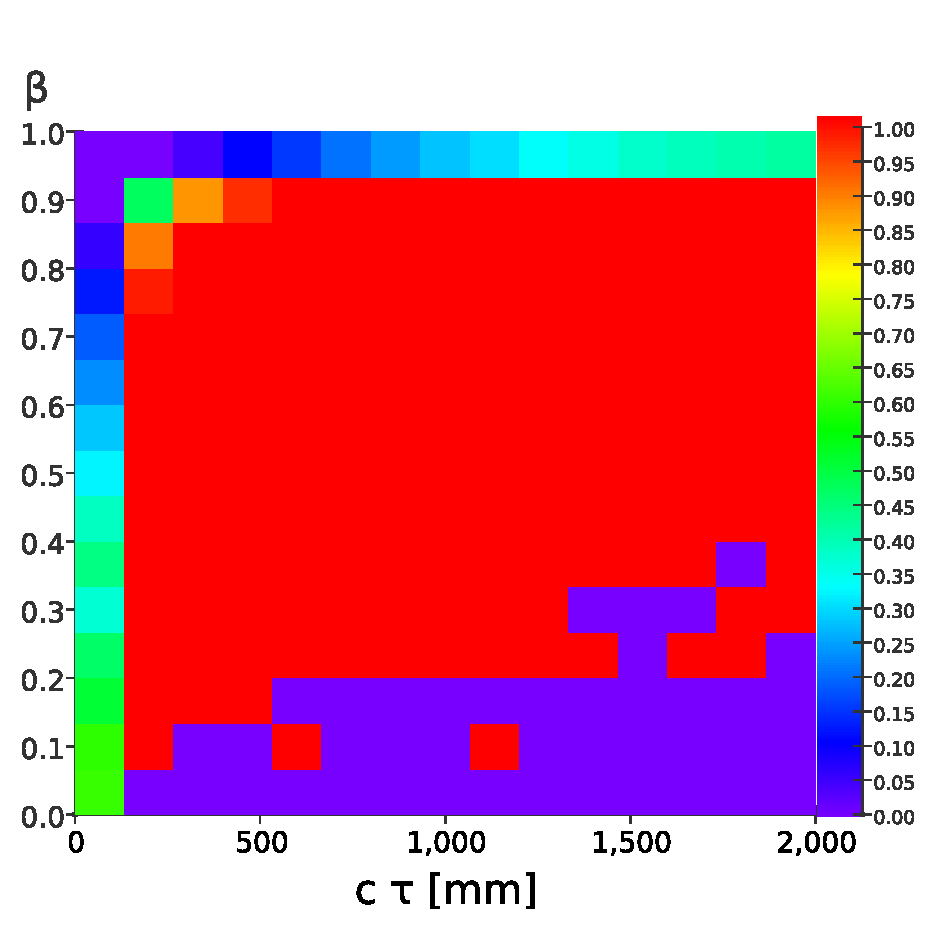
\includegraphics[width=0.41\textwidth]{effic20a_beta.pdf}\hfill
   }
   \subfigure[1000 ps] {
   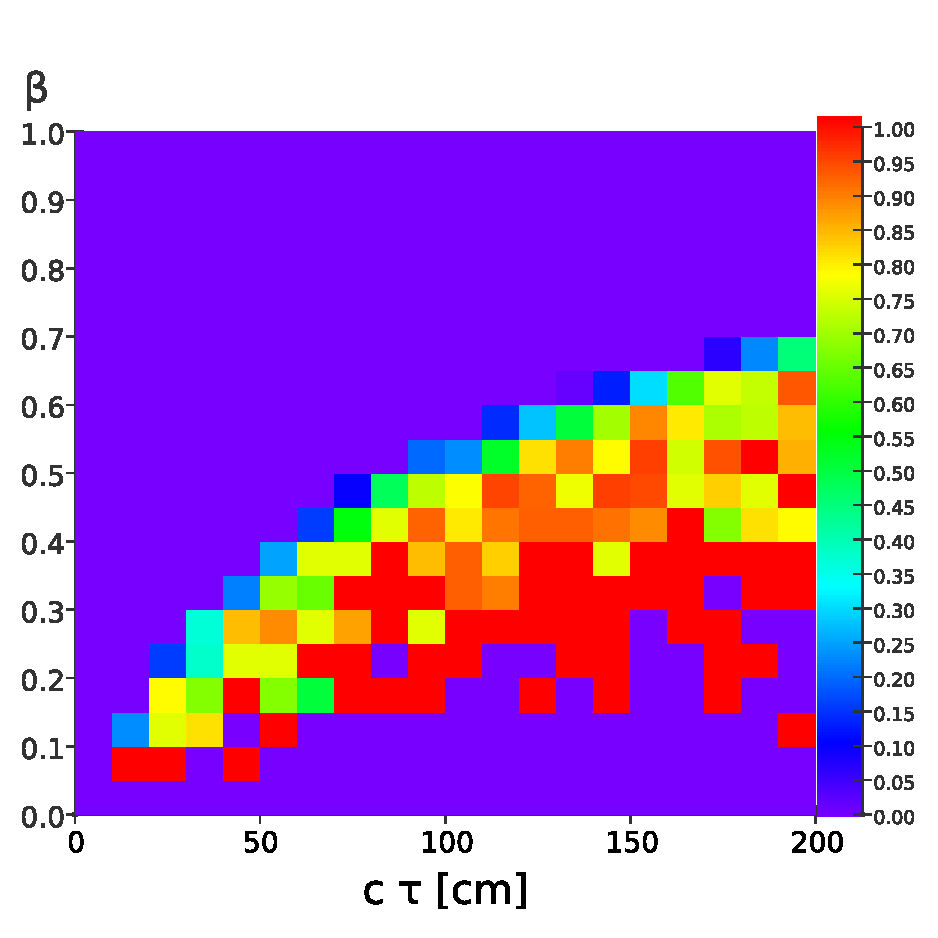
\includegraphics[width=0.41\textwidth]{effic1000a_beta.pdf}\hfill
   }

\end{center}
\caption{
The efficiency for the reconstruction of emerging jets using the timing layers with different timing resolutions.
The plot shows the efficiency as a function of $c\tau$ and the  particle velocity $\beta$
}
\label{fig:efficiency_beta}
\end{figure}



\end{document}
